\providecommand{\main}{../../..}
\documentclass[\main/main.tex]{subfiles}
\begin{document}

\subsection{Esercizio 3}
Si descriva brevemente il metodo della trasformazione inversa per enumerare le soluzioni paretiane, specificandone le condizioni di applicazione.

Si applichi tale metodo al seguente problema:

\begin{align*}
	\max f_1  = x_1 + x_2  \\
	\max f_2  = x_1 - x_2  \\
	x_1^2 + x_2^2 & \leq 1 \\
	x_1 \leq 0
\end{align*}

\subsection{Soluzione esercizio 3}

\subsubsection*{Metodo della trasformazione inversa}
Si determina l'inversa della funzione $f$, $\phi: F \rightarrow X$, si sostituisce $x = \phi(x)$ nei vincoli e quindi si ottiene il sottoinsieme $F^o$ degli impatti preferibili e da quest'ultimo si ottiene quindi la regione paretiana $X^o$. È applicabile solo quando $f \in \mathbb{R}^2$.

\subsubsection*{Determino l'inversa $\phi$}
\[
	\begin{cases}
		f_1  = x_1 + x_2 \\
		f_2  = x_1 - x_2
	\end{cases}
	\Rightarrow
	\begin{cases}
		f_1  = 2x_1 - f_2 \\
		x_2  = x_1 - f_2
	\end{cases}
	\Rightarrow
	\begin{cases}
		x_1  = \frac{f_1 + f_2}{2} \\
		x_2  = \frac{f_1 - 2f_2}{2}
	\end{cases}
\]

\subsubsection*{Sostituisco l'inversa nei vincoli}
\[
	\begin{cases}
		\left( \frac{f_1 + f_2}{2} \right)^2 + \left(\frac{f_1 - 2f_2}{2}\right)^2 \leq 1 \\
		\frac{f_1 + f_2}{2} \leq 0
	\end{cases}
	\Rightarrow
	\begin{cases}
		\left( f_1 + f_2 \right)^2 + \left(f_1 - 2f_2\right)^2 \leq 4 \\
		f_1 + f_2 \leq 0
	\end{cases}
\]

L'immagine della regione paretiana $F^o$ è l'insieme di punti che non ammettono altri punti nel quadrante in basso a sinistra, che in questo caso costituiscono il segmento evidenziato in rosso nella figura \ref{area_paretiana_3}.

\begin{figure}
	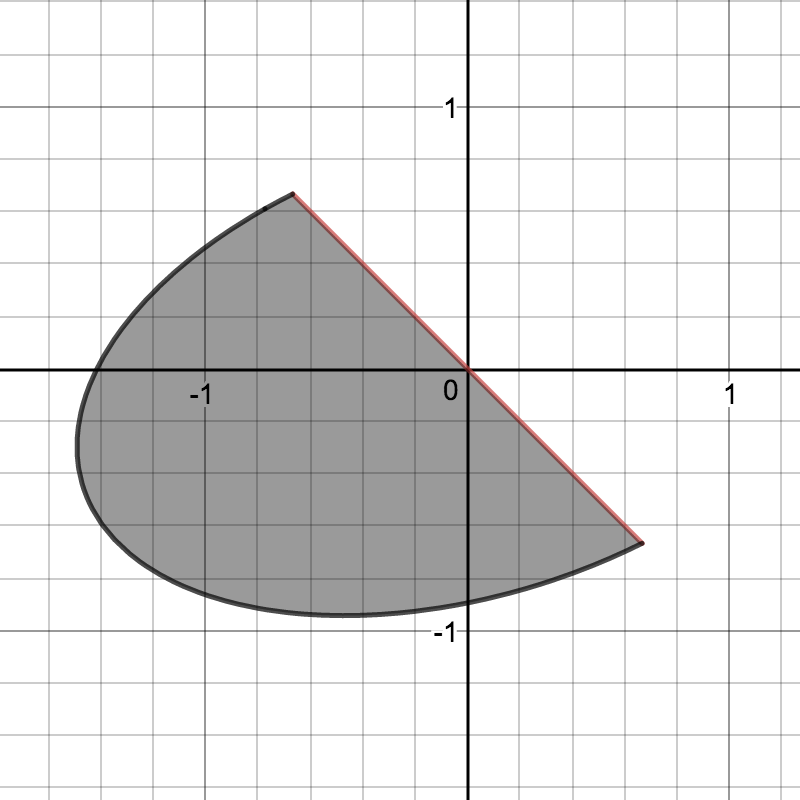
\includegraphics[width=0.3\textwidth]{14362016}
	\caption{In rosso l'immagine della regione paretiana.}
	\label{area_paretiana_3}
\end{figure}

La trasformazione inversa in questo caso è \textbf{lineare}, quindi anche la regione $X^o$ risulterà un segmento di retta.

Determino i punti di intersezione:

\[
	\begin{cases}
		\left( f_1 + f_2 \right)^2 + \left(f_1 - 2f_2\right)^2 = 4 \\
		f_1 + f_2 = 0
	\end{cases}
	\Rightarrow
	\begin{cases}
		\left( -f_2 + f_2 \right)^2 + \left(-f_2 - 2f_2\right)^2 = 4 \\
		f_1 = -f_2
	\end{cases}
	\Rightarrow
	\begin{cases}
		\left(-3f_2\right)^2 = 4 \\
		f_1 = -f_2
	\end{cases}
	\Rightarrow
	\begin{cases}
		9f_2^2 = 4 \Rightarrow \pm \frac{2}{3} \\
		f_1 = -f_2
	\end{cases}
\]

I due punti risultano essere quindi: $A = (\frac{2}{3}, -\frac{2}{3})$ e $B = (-\frac{2}{3}, \frac{2}{3})$.

Calcolo quindi i punti che determina il segmento della regione paretiana.

\[
	\begin{cases}
		x_1  = 0 \\
		x_2  = \frac{-3f_2}{2} = \pm 1
	\end{cases}
\]

Da cui i due punti che determinano il segmento della regione paretiana $X^o$ sono $C = (0, -1)$ e $D = (0, 1)$.

\begin{figure}
	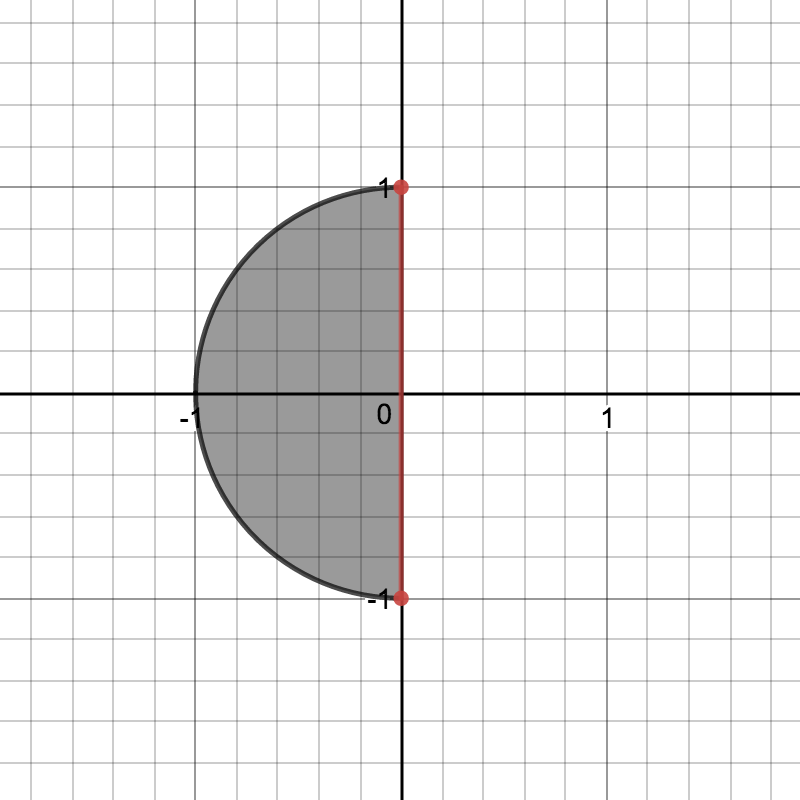
\includegraphics[width=0.3\textwidth]{14362016X}
	\caption{In rosso la regione paretiana.}
	\label{area_paretiana_4}
\end{figure}


\subsubsection*{Verifico i risultati ottenuti}
\begin{figure}
	\begin{subfigure}{0.30\textwidth}
		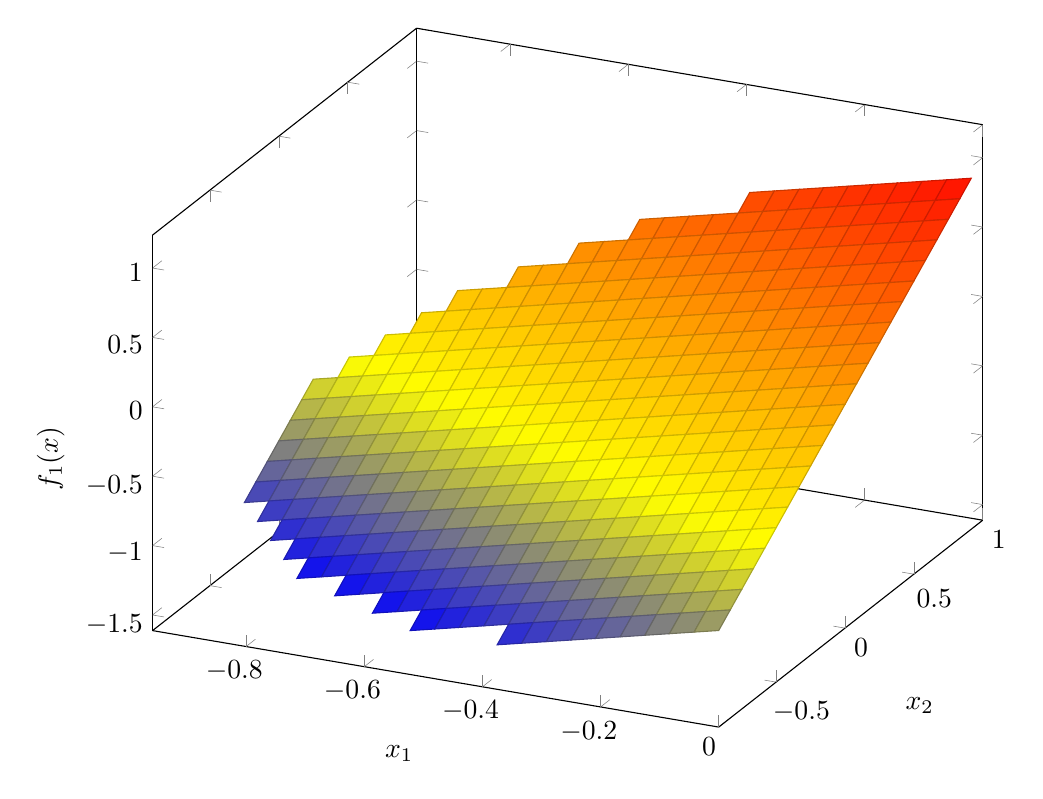
\begin{tikzpicture}
			\begin{axis}[
					width=\textwidth,
					xlabel=$x_1$,
					ylabel=$x_2$,
					zlabel=$f_1(x)$,
					domain=-1:0,
					y domain=-1:1
				]
				\addplot3[surf, unbounded coords=jump]
				{x^2 + y^2 <  1 ? x + y : NaN};
			\end{axis}
		\end{tikzpicture}
		\caption{L'indicatore $f_1(x)$}
	\end{subfigure}
	~
	\begin{subfigure}{0.30\textwidth}
		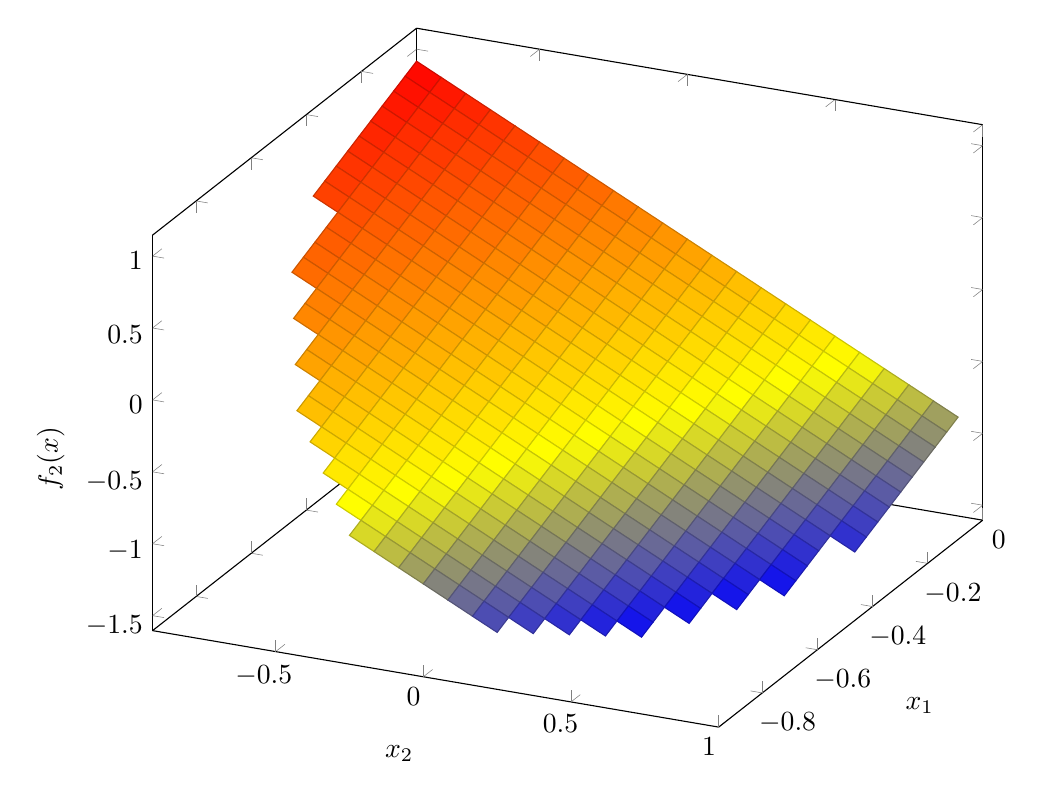
\begin{tikzpicture}
			\begin{axis}[
					width=\textwidth,
					xlabel=$x_2$,
					ylabel=$x_1$,
					zlabel=$f_2(x)$,
					domain=-1:1,
					y domain=-1:0
				]
				\addplot3[surf, unbounded coords=jump]
				{x^2 + y^2 <  1 ? y-x : NaN};
			\end{axis}
		\end{tikzpicture}
		\caption{L'indicatore $f_2(x)$}
	\end{subfigure}
	~
	\begin{subfigure}{0.30\textwidth}
		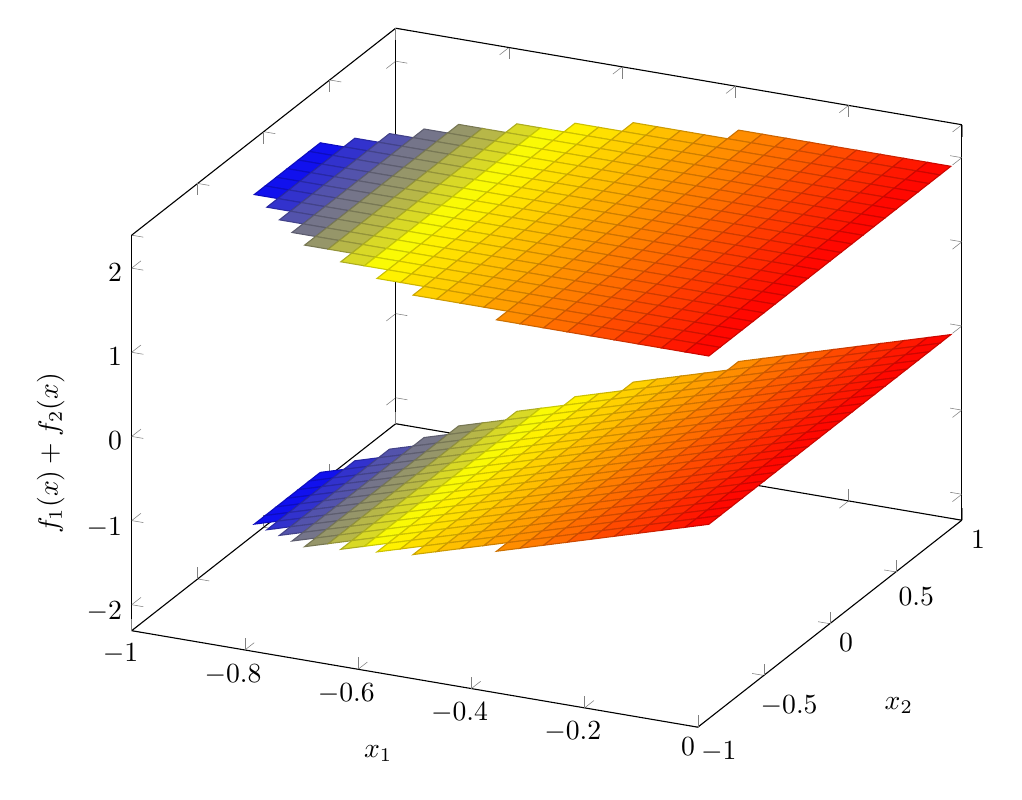
\begin{tikzpicture}
			\begin{axis}[
					width=\textwidth,
					xlabel=$x_1$,
					ylabel=$x_2$,
					zlabel=$f_1(x)+f_2(x)$,
					domain=-1:0,
					y domain=-1:1
				]
				\addplot3[surf, unbounded coords=jump]
				{x^2 + y^2 <  1 ? y+x + x-y : NaN};
				\addplot3[
					surf,
					point meta rel=per plot,
					point meta={x^2 + y^2 <  1 ? y+x + x-y : NaN}
				] {2};
			\end{axis}
		\end{tikzpicture}
		\caption{La somma degli indicatori}
	\end{subfigure}
\end{figure}

I due indicatori assumono valori nella stessa magnitudo nel dominio di definizione per cui, in questo caso, è possibile stimare il massimo dei due indicatori come il massimo della funzione ottenuta sommandoli. Il risultato ottenuto è coerente con la regione paretiana evidenziata.

\end{document}